% !TEX TS-program = pdflatex
% !TEX encoding = UTF-8 Unicode

% This is a simple template for a LaTeX document using the "article" class.
% See "book", "report", "letter" for other types of document.

\documentclass[11pt]{article} % use larger type; default would be 10pt

\usepackage[utf8]{inputenc} % set input encoding (not needed with XeLaTeX)

%%% PAGE DIMENSIONS
\usepackage{geometry} % to change the page dimensions
\geometry{a4paper} % or letterpaper (US) or a5paper or....

\usepackage{graphicx} % support the \includegraphics command and options

\usepackage{amssymb}
\usepackage{amsmath}
%%% PACKAGES
\usepackage{booktabs} % for much better looking tables
\usepackage{array} % for better arrays (eg matrices) in maths
\usepackage{paralist} % very flexible & customisable lists (eg. enumerate/itemize, etc.)
\usepackage{verbatim} % adds environment for commenting out blocks of text & for better verbatim
\usepackage{subfig} % make it possible to include more than one captioned figure/table in a single float
% These packages are all incorporated in the memoir class to one degree or another...

%%% HEADERS & FOOTERS
\usepackage{fancyhdr} % This should be set AFTER setting up the page geometry
\pagestyle{fancy} % options: empty , plain , fancy
\renewcommand{\headrulewidth}{0pt} % customise the layout...
\lhead{}\chead{}\rhead{}
\lfoot{}\cfoot{\thepage}\rfoot{}

%%% SECTION TITLE APPEARANCE
\usepackage{sectsty}
\allsectionsfont{\sffamily\mdseries\upshape} % (See the fntguide.pdf for font help)
% (This matches ConTeXt defaults)

%%% ToC (table of contents) APPEARANCE
\usepackage[nottoc,notlof,notlot]{tocbibind} % Put the bibliography in the ToC
\usepackage[titles,subfigure]{tocloft} % Alter the style of the Table of Contents
\renewcommand{\cftsecfont}{\rmfamily\mdseries\upshape}
\renewcommand{\cftsecpagefont}{\rmfamily\mdseries\upshape} % No bold!
\usepackage{graphicx}
\graphicspath{ {./pings/} }

\usepackage{amsmath}
\DeclareMathOperator*{\argmax}{arg\,max}
\DeclareMathOperator*{\argmin}{arg\,min}

\newcount\colveccount
\newcommand*\colvec[1]{
        \global\colveccount#1
        \begin{pmatrix}
        \colvecnext
}
\def\colvecnext#1{
        #1
        \global\advance\colveccount-1
        \ifnum\colveccount>0
                \\
                \expandafter\colvecnext
        \else
                \end{pmatrix}
        \fi
}

%%% END Article customizations

%%% The "real" document content comes below...

\title{Macro PS2}
\author{Michael B. Nattinger\footnote{I worked on this assignment with my study group: Alex von Hafften, Andrew Smith, and Ryan Mather. I have also discussed problem(s) with Emily Case, Sarah Bass, and Danny Edgel.}}

%\date{} % Activate to display a given date or no date (if empty),
         % otherwise the current date is printed 

\begin{document}
\maketitle
\section{Question 1}
\subsection{Part A}
%First we can solve the household side. 
%
%We can write our Bellman equation as follows, and then divide capital variables by A to normalize, yielding lowercase variables:
%\begin{align*}
%V(K) = &\max_{C,K',N} u(c,1-N) + \beta V(K')\\
%&\text{s.t. } K' = (1-\delta)K + Y - C \\
%&\text{and }Y = F(K,AN)\\
%\Rightarrow V(k) = &\max_{c,k',N} u(c,1-N) + \beta(1+g) V(k') \\
%&\text{s.t. } k' = (1-\delta)k + y - c \\
%&\text{and }y = F(k,N)\\
%\Rightarrow V(k) &= \max_{c,N} u(c,1-N) + \beta (1+g) V((1-\delta)K + F(K,AN) - c)
%\end{align*}
%Taking FOCs and applying the envelope condition we find:
%\begin{align*}
%0 &= u_1(c,1-N) - \beta(1+g) V'((1-\delta)k + F(k,N) - c)\\
%V'(k) &= \beta(1+g) V'((1-\delta)k + F(k,N) - c)(1-\delta + F_1(k,N))\\
%\Rightarrow V'(k) &=u_1(c,1-N) (1-\delta + F_1(k,N)) \\
%\Rightarrow u_1(c,1-N) &= \beta(1+g) u_1(c,1-N) (1-\delta + F_1((1-\delta)k + F(k,N) - c,N))\\
%\Rightarrow F_1((1-\delta)k + F(k,N) - c,N) &= \frac{1}{\beta(1+g)} - 1 + \delta
%\end{align*}
%\begin{equation}
%\Rightarrow F_1(k',N) = \frac{1}{\beta(1+g)} - 1 + \delta \label{eqn:FOC1}
%\end{equation}
%
%\begin{align*}
%0 &= -u_2(c,1-N) - \beta(1+g) V'((1-\delta)k + F(k,N) - c)(F_2(k,N))\\
%\Rightarrow u_2(c,1-N) &= - \beta(1+g) u_1(c,1-N) (1-\delta + F_1((1-\delta)k + F(k,N) - c,N))(F_2(k,N))
%\end{align*}
%\begin{equation}
%\frac{ u_2(c,1-N)}{u_1(c,1-N)} = - \beta(1+g)(1-\delta + F_1(K',AN))(AF_2(K,AN)) \label{eqn:FOC2}
%\end{equation}
%
%Equations (\ref{eqn:FOC1}), (\ref{eqn:FOC2}), and our feasibility constraint $(k' = (1-\delta)k +F(k,N) - c)$ form our difference equations for $(k',c,n)$ (3 eqns in 3 unknowns).
%
%Now we must solve the firm side. 
%
%The firm maximizes profits:
%\begin{align*}
%\max_{k^d,n^d} \sum_{t=1}^{\infty} 
%\end{align*} 

We will write down the equations to characterize the system, normalize by $A$, and then solve for our difference equations. 

Households maximize utility subject to their budget constraints (note: I denote $w_t$ as normalized wages, $W_t/A_t$ throughout):

\begin{align*}
&\max_{\{C_t,I_t,N_t,K_t\}_{t=0}^{\infty}} \sum_{i=0}^{\infty}\beta^t u(C_t,1-N_t)\\
&\text{s.t. } \sum_{t=0}^{\infty} p_t (C_t + I_t) =  \sum_{t=0}^{\infty} p_t(r_tK_t + w_tA_tN_t) + \Pi_0\\
&\text{and } K_{t+1} = (1-\delta) K_t+ I_t
\end{align*}

Firms maximize profits:
\begin{align*}
\max \Pi_0 &=\sum_{t=0}^{\infty}p_t(Y_t -r_tK_t^d - w_t A_tN_t^d)\\
\text{s.t. } Y_t &= F(K_t,A_tN_t^d)
\end{align*}

Now we normalize. Let lowercase $x_t = X_t/A_t$:

HH:
\begin{align*}
&\max_{\{c_t,i_t,n_t,k_t\}_{t=0}^{\infty}} \sum_{i=0}^{\infty}\beta^t u(c_tA_t,1-N_t)\\
&\text{s.t. } \sum_{t=0}^{\infty} p_t (c_t + i_t) =  \sum_{t=0}^{\infty} p_t(r_tk_t + w_tN_t) + \Pi_0\\
&\text{and } k_{t+1}(1+g) = (1-\delta) k_t+ i_t
\end{align*}

Firms:
\begin{align*}
\max \Pi_0 &=\sum_{t=0}^{\infty}p_t(y_t -r_tk_t^d - w_t N_t^d)\\
\text{s.t. } y_t &= F(k_t^d,N_t^d)
\end{align*}

Now we begin to solve. We will start with the firm side:

\begin{align*}
F_k(k_t^d,N_t^d) &= r_t\\
F_N(k_t^d,N_t^d) &= w_t\\
\Rightarrow F(k_t^d,N_t^d) - F_k(k_t^d,N_t^d) r_t - F_N(k_t^d,N_t^d) w_t &= 0 \\\Rightarrow \Pi_0 &= 0.
\end{align*}

Now we move to the HH side. Our HH problem can be reduced to the following:
\begin{align*}
&\max_{c_t,n_t} \sum_{i=1}^{\infty}\beta^t u(A_tc_t,1-N_t)\\
&\text{s.t. } \sum_{t=0}^{\infty} p_t ( c_t + k_{t+1} - [r_t + (1-\delta)]k_t - w_tN_t ) = 0
\end{align*}
Taking first order conditions of our lagrangian:

\begin{align*}
A_t\beta^tu_c(c_tA_t,1-N_t) &= \lambda p_t\\
A_{t+1}\beta^{t+1}u_c(c_{t+1}A_{t+1},1-N_{t+1}) &= \lambda p_{t+1}\\
\Rightarrow (1+g)\frac{\beta u_c(c_{t+1}A_{t+1},1-N_{t+1})}{ u_c(c_tA_t,1-N_t)} &= \frac{p_{t+1}}{p_t}\\
-\beta^tu_n(c_tA_t,1-N_t) &= \lambda p_tw_t \\
-\beta^{t+1}u_n(c_{t+1}A_{t+1},1-N_{t+1}) &= \lambda p_{t+1}w_{t+1}\\
\Rightarrow \frac{\beta u_n(c_{t+1}A_{t+1},1-N_{t+1}) }{u_n(c_tA_t,1-N_t)} &= \frac{p_{t+1} w_{t+1}}{p_t w_t}\\
p_t &= p_{t+1}(r_{t+1} + 1-\delta)
\end{align*}

In the competitive equilibrium, markets clear:
\begin{align*}
k_t^d &= k_t\\
N_t^d &= N_t\\
c_t + k_{t+1}(1+g) - (1-\delta)k_{t} &= F(k_t^d,N_t^d)
\end{align*}

The equations that pin down $C_0,N_0,w_0,r_0$ in the balanced growth path are the following four equations:

\begin{align*}
F_k(k_0,N_0) &= r_0\\
F_N(k_0,N_0) &= w_0\\
A_0 u_c (c_0 A_0, 1-N_0) &= - u_n (c_0A_0,1-N_0) / w_0\\
c_0 + k_0(1+g) - (1-\delta)k_0 &= F(k_0,N_0).
\end{align*}
This is 4 equations in 4 unknowns. Note that this final equation comes from the law of motion of capital, but in the balanced growth path $k_0 = k_1$. We can then solve for $C_0 = c_0A_0$.


\subsection{Part B}
In general, the following equations form our law of motion for the system.
\begin{align}
(1+g)\frac{\beta u_c(c_{t+1}A_{t+1},1-N_{t+1})}{ u_c(c_tA_t,1-N_t)} &= \frac{p_{t+1}}{p_t} \label{ceuler} \\
\frac{\beta u_n(c_{t+1}A_{t+1},1-N_{t+1}) }{u_n(c_tA_t,1-N_t)} &= \frac{p_{t+1} w_{t+1}}{p_t w_t}\label{neuler}\\
p_t &= p_{t+1}(r_{t+1} + 1-\delta) \label{arbitrage} \\ 
F_k(k_t,N_t) &= r_t\\
F_N(k_t,N_t) &= w_t \\
c_t + k_{t+1}(1+g) - (1-\delta)k_{t} &= F(k_t,N_t)
\end{align}

If preferences are of the form:
\begin{align*}
u(C,1-N) &= \frac{C^{1-\gamma}}{1-\gamma}h (1-N), \gamma >0, \gamma \neq 1\\
& logC + h(1-N), \gamma = 1
\end{align*}

First, assume $\gamma \neq 1.$ Then, equation (\ref{ceuler}), (\ref{neuler}) becomes the following:
\begin{align}
\beta (1+g)^{1-\gamma}\left( \frac{c_{t+1}}{c_t}\right)^{-\gamma} \frac{h(1-N_{t+1})}{h(1-N_t)} &= \frac{p_{t+1}}{p_t} \label{newceuler} \\
\beta (1+g)^{1-\gamma}\left( \frac{c_{t+1}}{c_t}\right)^{1-\gamma} \frac{h'(1-N_{t+1})}{h'(1-N_t)} &= \frac{p_{t+1}w_{t+1}}{p_tw_t} \label{newneuler}
\end{align}

Note that if $\gamma=1,$ we get the same results as (\ref{newceuler}), (\ref{newneuler}).

Now, we can find the balanced growth path as follows. We note that inflation will occurn in the balanced growth path, and we can define $\pi_t = \frac{p_{t+1}}{p_t}$, and solve for $\bar{\pi}$. Equations (\ref{newceuler}), (\ref{newneuler}), (\ref{arbitrage}) imply:
\begin{align*}
\beta(1+g)^{1-\gamma} &= \bar{\pi}\\
\frac{w_{t+1}}{w_t} = 1 \Rightarrow w_t = \bar{w} = w_{t+1} \\
\frac{1}{\bar{\pi}} + \delta - 1 &= \bar{r}
\end{align*}

We then have the following system of equations which can be solved to find the balanced growth path of the economy:

\begin{align}
F_k(\bar{k},\bar{N}) &= \bar{r} \label{ss1}\\
F_N(\bar{k},\bar{N}) &= \bar{w}\label{ss2} \\
\bar{c} + (g+\delta)\bar{k} &= F(\bar{k},\bar{N}) \label{ss3}
\end{align}

Equations (\ref{ss1}), (\ref{ss2}), and (\ref{ss3}) form 3 equations in 3 unknowns (initial capital, $k_0 = \bar{k}$, is given). By the Inada conditions on $F$ and its continuous differentiability, the solution to these equations exists and is unique. Therefore, there will be a balanced growth path.

\subsection{Part C}
We solved for our balanced growth path in this case by taking capital as given - exogenous. If the parameters change, we would not be able to determine the effect on both capital and consumption in the balanced growth path unless we were given the new capital level for the balanced growth path.

Moreover, we cannot summarize the information in the same way as before without further information because now labor supply can move endogenously. We will not know the impact on labor supply, which will affect the response of the economy to the change in $\delta$. For instance, if the labor supply increases sufficiently, then consumption will shoot up, resulting in a new steady state with higher consumption levels. However, if the labor supply decreases sufficiently, then consumption will fall immediately and the new steady state the economy ends up at may have lower consumption levels. The overall effect on consumption is therefore indeterminate due to the labor supply dynamics.

% write about how k is exogenously determined here. Later, in D, you can actually solve for 

\subsection{Part D}

Let labor supply be inelastic. Then, there is no disutility from working so $n_t = 1 \forall t.$ Most of our equations from before still hold. Specifically, the following conditions must still hold:

\begin{align}
\beta (1+g)^{1-\gamma}\left( \frac{c_{t+1}}{c_t}\right)^{-\gamma} &= \frac{p_{t+1}}{p_t} \label{eq1} \\
p_t &= p_{t+1}(r_{t+1} + 1-\delta) \label{eq2}\\ 
c_t + k_{t+1}(1+g) - (1-\delta)k_{t} &= f(k_t) \label{eq3}
\end{align}

We now can redefine $f(k) = F (k,1)$ and we have, also from before,

\begin{equation}
f'(k_t) = r_t \label{eq4}
\end{equation}

Finally, we can pin down wage by the zero profit condition we solved for:

\begin{align}
w_t &= f(k_t)  - f'(k_t)r_t \label{eq5}
\end{align}

Equations (\ref{eq1}), (\ref{eq3}) form our equations governing the law of motion of capital and consumption, and equations (\ref{eq2}), (\ref{eq4}), and (\ref{eq5}) pin down the evolution of wages, inflation, and the rental price of capital over time.

Combining equations  (\ref{eq1}), (\ref{eq3}) allows us to solve for the balanced growth path of capital and consumption. Note that we could not solve for the steady state value of capital in this way before due to the endogenous movement of labor, as we described in part C.

\begin{align*}
\beta(1+g)^{1-\gamma} &= \bar{\pi}\\
\frac{1}{\bar{\pi}} + \delta - 1 &= \bar{r} \\
 f'^{-1}(\bar{r}) &= \bar{k} \\
 f(\bar{k})  - f'(\bar{k})\bar{r} &= \bar{w} \\
f(\bar{k}) - (g+\delta) \bar{k} &= \bar{c}
\end{align*}

\subsection{Part E}
Let $g$ fall. First, we will consider long term dynamics (changes in the balanced growth path), then we will consider how the economy transitions in the short run.

$g$ falls implies $\bar{\pi}$ falls, so $\bar{r}$ rises. Thus, $\bar{k}$ falls. Now, consider $\bar{c}$. As $\bar{k}$ falls, $f(\bar{k})$ falls. However, for the $-(g+\delta)$ term, $-(g+\delta)$ rises and $\bar{k}$ rises so the effect of this term is an increase, and therefore the effect on $\bar{c}$ as a whole is indeterminate.

Initially, when $g$ falls, capital is fixed. Consumption falls to compensate, finding the new saddle path. The economy progresses along the new saddle path until it reaches the new balanced growth path.

\subsection{Part F}
Output saved on the balanced growth path is production less consumption, i.e. $\bar{s} = f(\bar{k}) - \bar{c} = (g+\delta) \bar{k}$. 

\begin{align*}
\frac{\partial \bar{s}}{\partial g} &= \bar{k} + (g+\delta ) \frac{\partial \bar{k}}{\partial g}\\
 \frac{\partial \bar{k}}{\partial g} &= \frac{\partial }{\partial g} f'^{-1}(\bar{r}) = (f'^{-1})'(\bar{r}) \frac{\partial \bar{r}}{\partial g}\\
\frac{\partial \bar{r}}{\partial g} &= - \frac{1}{(\bar{\pi})^2} \frac{\partial \bar{\pi}}{\partial g} \\
\frac{\partial \bar{\pi}}{\partial g} &= (1-\gamma)\beta (1+g)^{-\gamma} \\
\Rightarrow \frac{\partial \bar{s}}{\partial g} &=  \bar{k} - \frac{ (g+\delta )(f'^{-1})'(\bar{r})}{(\bar{\pi})^2}(1-\gamma)\beta (1+g)^{-\gamma} \\
\end{align*}
\begin{align}
\Rightarrow \frac{\partial \bar{s}}{\partial g} &=  \bar{k} - \left( \frac{g+\delta}{(1+g)^{\gamma}} \right) \frac{(1-\gamma)\beta (f'^{-1})'(\bar{r})}{(\bar{\pi})^2}
\end{align}

Therefore, savings will rise as $g$ increases if $ \bar{k} > \left( \frac{g+\delta}{(1+g)^{\gamma}} \right) \frac{(1-\gamma)\beta (f'^{-1})'(\bar{r})}{(\bar{\pi})^2},$ which will occur with certainty if $(f'^{-1})'(\bar{r})\leq0.$

For $F(k,N) = k^{\alpha} N^{1-\alpha},$ $f(k) = k^{\alpha} \Rightarrow f'(k) = \alpha k^{\alpha - 1} \Rightarrow f'^{-1}(r) = \left(\frac{r}{\alpha}\right)^{1/(\alpha-1)} \Rightarrow (f'^{-1})'(r) = \left( \frac{1}{\alpha - 1}\right) \left(\frac{r}{\alpha}\right)^{(1/(\alpha-1)) - 1}. $ Since $\alpha<1,  \left( \frac{1}{\alpha - 1}\right) <0$ so $(f'^{-1})'(r)<0$, so $\frac{\partial \bar{s}}{\partial g}>0$. Therefore, for the Cobb-Douglas production function, balanced growth path savings increases as $g$ rises.

\section{Question 2}
\subsection{Part A}
The consumer chooses consumption to maximize expected utility:
\begin{align*}
\max_{\{c_t\}_{t=0}^{\infty}} E\sum_{t=0}^{\infty}\beta^t \frac{c_t^{1-\gamma}}{1-\gamma}\\
\text{s.t. } x_t \leq A_{t-1}(x_{t-1} - c_{t-1}),
\end{align*}

where $A_t$ are i.i.d. shocks with possible values $A_h,A_l$. Therefore, our space consists of $A_t = y \in \{ A_h,A_l \}; Y = \{ \emptyset, \{A_h\},\{ A_l\}, \{ A_h,A_l\}\}; Q = \Pi = \begin{bmatrix} \pi & (1-\pi) \\ \pi & (1-\pi)\end{bmatrix}$. The expectations operator is the probability-weighted average of total discounted utility across all possibilities of future shocks. 
\subsection{Part B}
We will write the bellman operator in the following form:
\begin{align*}
V(As) &= \max_{s'} \frac{(As - s')^{1-\gamma}}{1-\gamma} + \beta EV(As')\\
&= \max_{s'} \frac{(As - s')^{1-\gamma}}{1-\gamma} + \beta (\pi V(A'_h s') + (1-\pi) V(A'_l s' )),
\end{align*}
where $s_t := x_t - c_t$. Our value is dependent on the value we have when making our decision, i.e. post shock-realization, so our state variable for the Bellman equation is $A_{t-1}s_{t-1} = x_t$.

%(prove the optimal value function is continuous, increasing, and concave)

The utility function is concave, increasing, and continuous. The feasible set is convex, continuous, and nonempty. Furthermore, $0<\beta<1$. Moreover, we will show below that we can treat $u$ such that it is bounded. Given all of these, we know that our optimal value function is continuous, increasing, and concave.

As I mentioned, we can treat $u$ such that it is bounded. The reason for this stems from the fact that we are given that $A_l<A_h<\frac{1}{\beta} \Rightarrow A_l \beta < A_h \beta <1$.Therefore, due also to the concavity of $u$, the discounted present value of saving your money and spending later, even if one were to draw $A_h$ every single time (i.e. even if $\pi=1$) declines with the time horizon at least at the rate $A_h \beta <1$, so the value function is guaranteed to be finite even though $u$ is not itself bounded from above. 

\subsection{Part C}
To solve the Bellman, we will take first order conditions, 

\begin{align*}
(As - s')^{-\gamma}&= \beta(\pi V'(A'_hs') + (1-\pi)V'(A'_l s'))\\
V'(As) &= (As -s')^{-\gamma}\\
\Rightarrow (As - s')^{-\gamma}&= \beta(\pi (A'_hs'-s''_h)^{-\gamma} + (1-\pi)(A'_l s'-s''_l)^{-\gamma})
\end{align*}

We will guess and verify that our optimal policy function is to save a constant percentage of our wealth.

Let $As-s' = pAs$. Then, our $p$ must satisfy the following (note: $p>0$ by our Inada conditions):
\begin{align*}
(pAs)^{-\gamma} &= \beta(\pi (pA_hs')^{-\gamma} + (1-\pi)(pA_ls')^{-\gamma} )\\
\Rightarrow (pAs)^{-\gamma} &= \beta \pi (pA_h(1-p)As)^{-\gamma} + \beta (1-\pi) (pA_l(1-p)As)^{-\gamma}\\
\Rightarrow  (pAs)^{-\gamma} &= \beta \pi ((p - p^2)A_hAs)^{-\gamma} + \beta (1-\pi) ((p - p^2)A_lAs)^{-\gamma} \\
\Rightarrow p^{-\gamma} &= \beta (p - p^2)^{-\gamma} (\pi A_h^{-\gamma} + (1-\pi) A_l^{-\gamma})\\
\Rightarrow (1-p) &= (\beta (\pi A_h^{-\gamma} + (1-\pi) A_l^{-\gamma}))^{1/\gamma} \\
\Rightarrow p &= 1 - (\beta (\pi A_h^{-\gamma} + (1-\pi) A_l^{-\gamma}))^{1/\gamma}.
\end{align*}

Therefore, saving a constant fraction of our wealth ($1-p =   (\beta (\pi A_h^{-\gamma} + (1-\pi) A_l^{-\gamma}))^{1/\gamma}$) is the optimal policy function.

\subsection{Part D}
From the following facts (the utility function is concave, increasing, and continuously differentiable; the feasible set is convex, compact, monotone, and nonempty; furthermore, $0<\beta<1$; moreover, we can treat $u$ such that it is bounded), we know that the consumption sequence generated by this policy function is the same as the original sequence problem.

\section{Question 3}
\subsection{Part A}
First we will derive the equations to form our model, then use the derived equations in Matlab to determine the optimal allocation.

Our Bellman equation is the following:
\begin{align*}
V(k) &= \max_{k'} \frac{(zk^{0.35} + (1-\delta)k - k')^{1-\gamma}}{1-\gamma} +\beta V(k')
\end{align*}

We take FOCs and apply the envelope theorem:
\begin{align*}
\beta V'(k') &=(zk^{0.35} + (1-\delta)k - k')^{-\gamma} \\
V'(k) &= (zk^{0.35} + (1-\delta)k - k')^{-\gamma}(0.35zk^{-0.65} +(1-\delta)) \\
\Rightarrow (zk^{0.35} + (1-\delta)k - k')^{-\gamma} &= \beta (zk'^{0.35} + (1-\delta)k' - k'')^{-\gamma}(0.35zk'^{-0.65} +(1-\delta))\\
\Rightarrow c^{-\gamma} &= c'^{-\gamma} \beta(0.35zk'^{-0.65}+(1-\delta))
\end{align*}
This, along with the law of motion of capital $k' = zk^{0.35} +(1-\delta)k - c$, forms our difference equations for $k,c$.

We can solve for the steady state as follows:

\begin{align*}
\frac{1}{\beta} &= 0.35z\bar{k}^{-0.65} +1 - \delta\\
\Rightarrow \bar{k} &= \left(\frac{\frac{1}{\beta}-1+\delta}{0.35z}\right)^{1/(-0.65)}\\
\Rightarrow \bar{c} &= z\bar{k}^{0.35} - \delta \bar{k}
\end{align*}

Finally, we can solve for our phase diagram lines:

\begin{align*}
\Delta c= 0 \Rightarrow \frac{1}{\beta} &= 0.35z(zk^{0.35} + (1-\delta)k - c )^{-0.65} + 1 - \delta\\
c&= zk^{0.35} + (1-\delta)k -\left(\frac{\frac{1}{\beta} - 1 + \delta}{0.35 z}\right)^{1/(-0.65)}\\
\Delta k = 0 \Rightarrow c &= zk^{0.35} - \delta k
\end{align*}

We will solve the value function numerically by iterating over the value function.

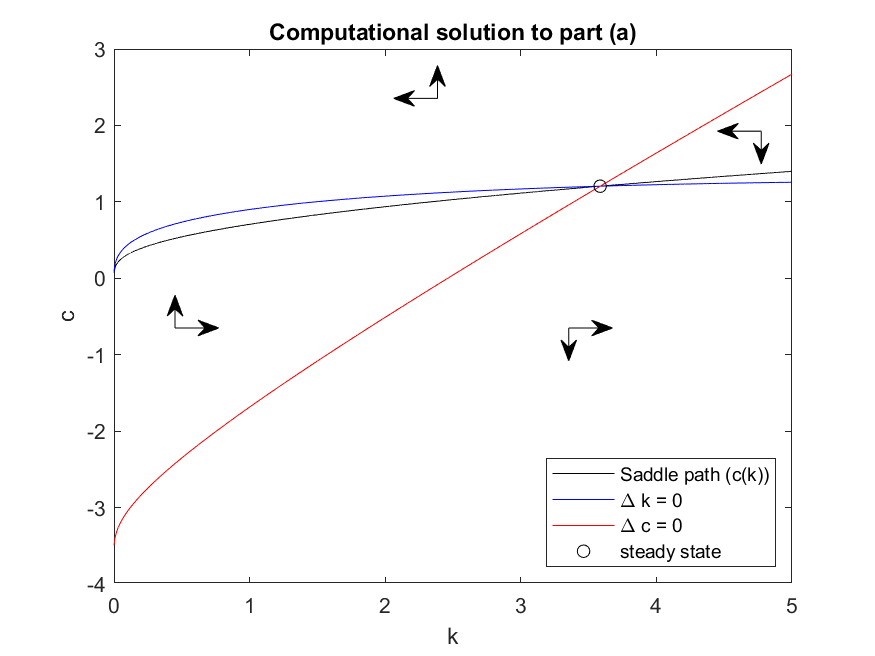
\includegraphics{partA}

As we can see, the computational saddle path is always positive and passes exactly through our steady state. We can also show our numerical solution for the value function, and $k'$ chosen as a function of $k$:

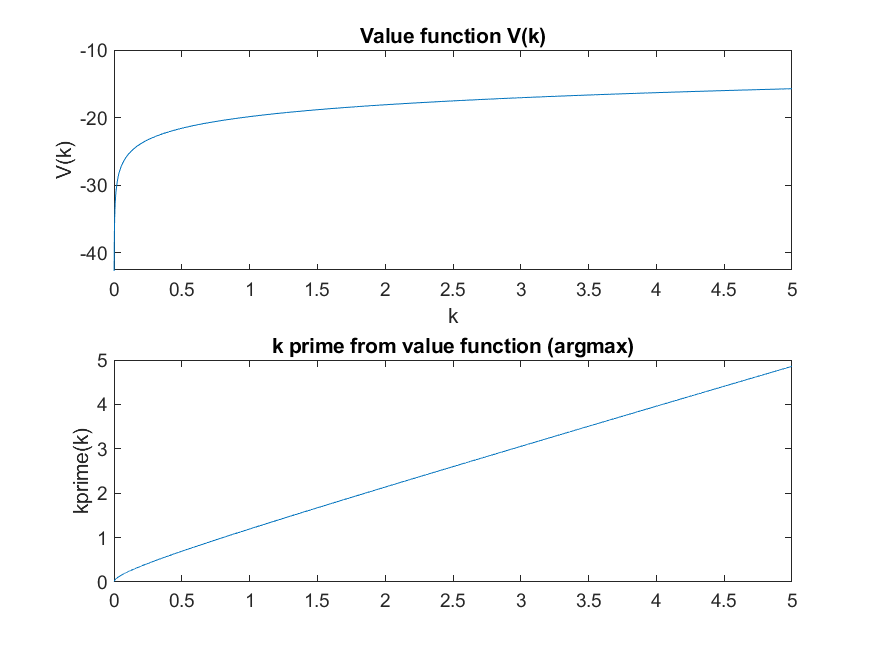
\includegraphics{partA2}

Our value function is clearly increasing, continuous, and concave in $k$. Our policy function $k'$ is increasing and nearly linear, with a slight concavity.

\subsection{Part B}

From our calculations in part (a), we know that the phase diagram lines are not affected by $\gamma$, so they will be unaffected by the parameter change. Furthermore, this also means that the steady state value will be unaffected. The reason for this is that the intertemporal elasticity of substitution does not affect the efficiency of capital, the labor supply decision (as there is no disutility of labor), the discount rate, or the depreciation rate, so the $\Delta c = 0,\Delta k = 0$ lines are unaffected by the change of intertemporal elasticity of substitution. However, this does not mean that our system as a whole will be unaffected - our decision rule (saddle) will be affected by the change in intertemporal elasticity of substitution. We will show this below.

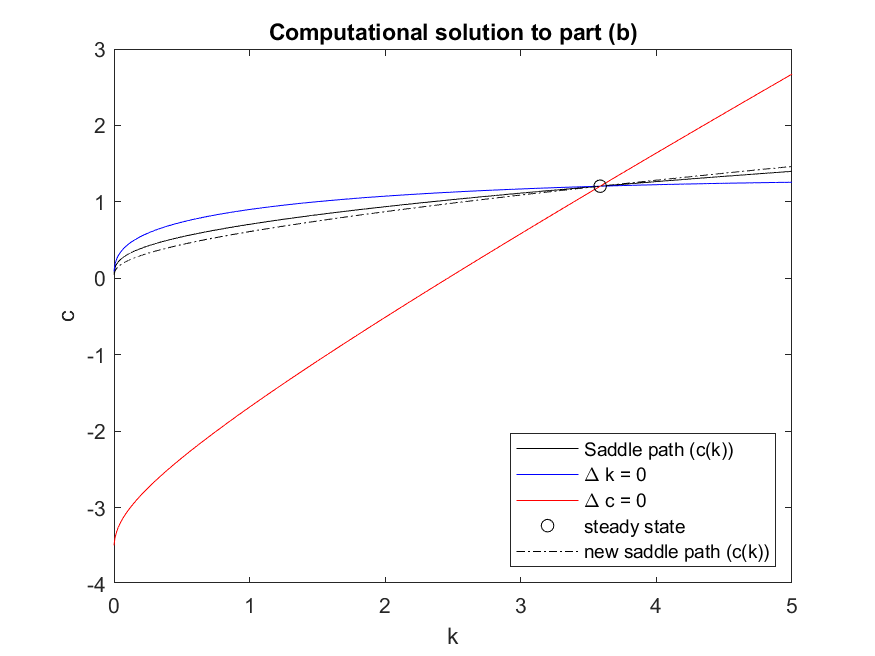
\includegraphics{partB}

As was predicted from our equations, the change in the $\gamma$ parameter results in a change in our decision rule (saddle), but not a mechanical change in our $\Delta c,\Delta k$ lines and therefore our steady state is unaffected. We can investigate the effect of the parameter change on our policy variables as well:

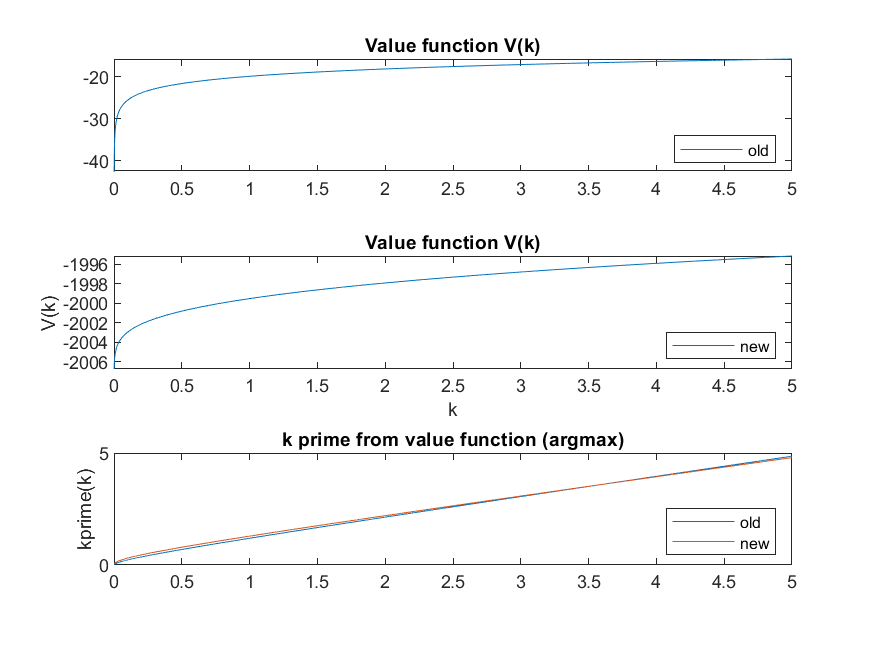
\includegraphics{partB2}

The value function with the new parameterization has a much lower value, which is to be expected due to the exponent on the flow utility function changing dramatically, and its shape is similar but a bit steeper than before. Still, the policy function $k'(k)$ is very similar to before, but the slight difference results in the difference in saddle path that we saw above.

\subsection{Part C}

Total factor productivity (TFP,$z$) does affect our steady state values and $\Delta c = 0,\Delta k = 0$ lines as the technological improvement yields mechanical improvements into our consumption and capital production frontiers. In other words, our capital is more effective, so we are able to produce more consumption and future capital goods given a current capital level. As such, the economy can sustain a higher level of both consumption and capital levels. Therefore, the steady state levels of consumption and capital will increase.

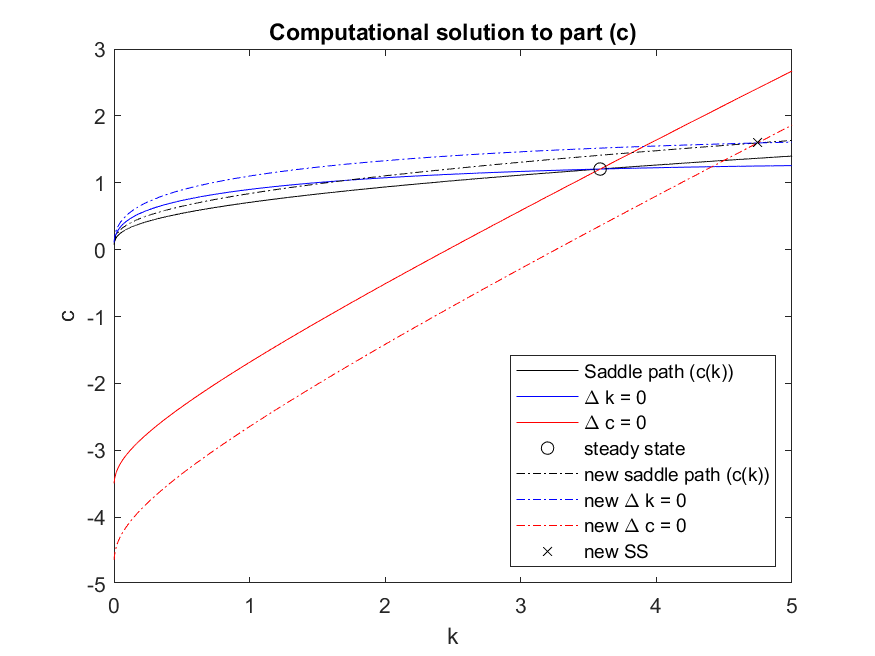
\includegraphics{partC}

We can also investigate the effect of the new parameterization on the policy variables:

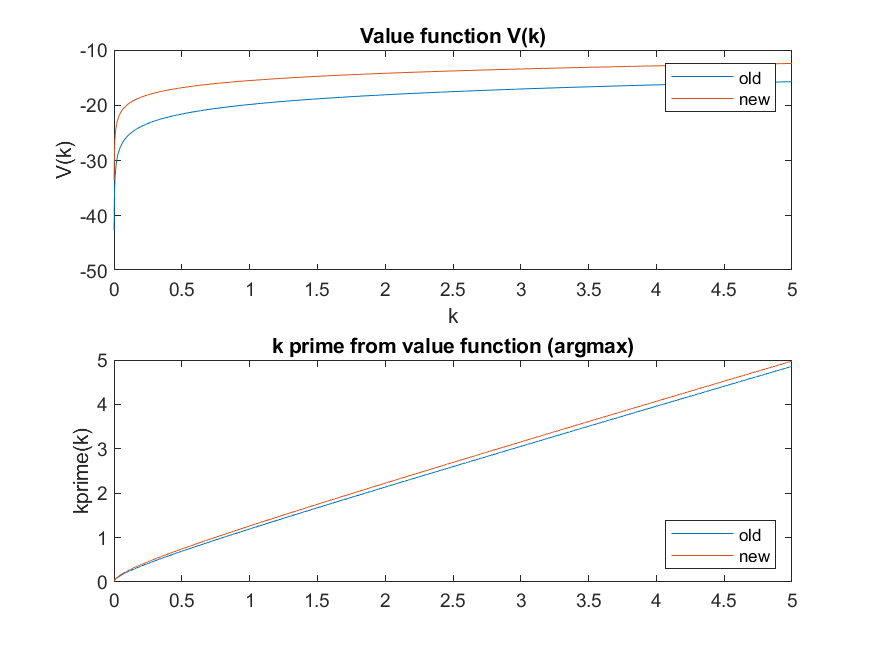
\includegraphics{partC2}

We can see that our value function has shifted up, which is because we are better off since our capital is more productive. Additionally, our decision rule $k'(k)$ has shifted up as well, as we are producing more with the capital we are given, and thus will always choose to keep more capital for the future.

When the transition occurs, production will jump up, but current capital levels are already fixed so consumption jumps to a higher level. It wil jump exactly to the new saddle path. The economy will then proceed along that saddle path towards the new steady state, which it will reach in the limit as $t\rightarrow \infty$. We will plot this transition below.

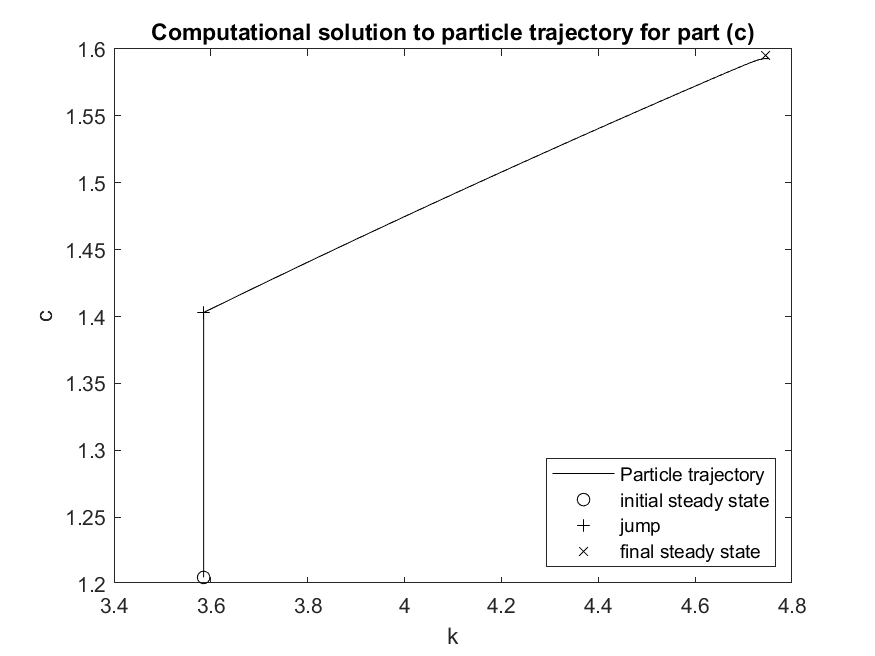
\includegraphics{traj}

As expected, our economy immediately jumps onto the new saddle path, and moves along that path to the new steady state.
\end{document}
